% !TEX TS-program = pdflatex
% !TEX encoding = UTF-8 Unicode

\documentclass[a4paper, titlepage=false, parskip=full-, 10pt]{scrartcl}

\usepackage[utf8]{inputenc}
\usepackage[T1]{fontenc}
\usepackage[english, ngerman]{babel}
\usepackage{babelbib}
\usepackage{hyperref}
\usepackage{listings}
\usepackage{framed}
\usepackage{color}
\usepackage{graphicx}
\usepackage[normalem]{ulem}
\usepackage{cancel}
\usepackage{amsmath}
\usepackage{amssymb}
\usepackage{amsthm}
\usepackage{algorithm}
\usepackage{algorithmic}
\usepackage{geometry}
\usepackage{subfigure}
\geometry{a4paper, top=20mm, left=35mm, right=25mm, bottom=40mm}

\newcounter{tasknbr}
\setcounter{tasknbr}{1}
\newenvironment{task}[1]{{\bf Aufgabe \arabic {tasknbr}\stepcounter{tasknbr}} (#1):\begin{enumerate}}{\end{enumerate}}
\newcommand{\subtask}[1]{\item[#1)]}

% Listings -----------------------------------------------------------------------------
\definecolor{red}{rgb}{.8,.1,.2}
\definecolor{blue}{rgb}{.2,.3,.7}
\definecolor{lightyellow}{rgb}{1.,1.,.97}
\definecolor{gray}{rgb}{.7,.7,.7}
\definecolor{darkgreen}{rgb}{0,.5,.1}
\definecolor{darkyellow}{rgb}{1.,.7,.3}
\lstloadlanguages{C++,[Objective]C,Java}
\lstset{
escapeinside={§§}{§§},
basicstyle=\ttfamily\footnotesize\mdseries,
columns=fullflexible, % typewriter font look better with fullflex
keywordstyle=\bfseries\color{blue},
% identifierstyle=\bfseries,
commentstyle=\color{darkgreen},      
stringstyle=\color{red},
numbers=left,
numberstyle=\ttfamily\scriptsize\color{gray},
% stepnumber=5,
% numberfirstline=true,
breaklines=true,
% prebreak=\\,
showstringspaces=false,
tabsize=4,
captionpos=b,
% framexrightmargin=-.2\textwidth,
float=htb,
frame=tb,
frameshape={RYR}{y}{y}{RYR},
rulecolor=\color{black},
xleftmargin=15pt,
xrightmargin=4pt,
aboveskip=\bigskipamount,
belowskip=\bigskipamount,
backgroundcolor=\color{lightyellow},
extendedchars=true,
belowcaptionskip=15pt}

%% Enter current values here: %%
\newcommand{\lecture}{Algorithmische Geometrie SS15}
\newcommand{\tutor}{}
\newcommand{\assignmentnbr}{12}
\newcommand{\students}{Julius Auer, Alexa Schlegel}
%%-------------------------------------%%

\begin{document}  
{\small \textsl{\lecture \hfill \tutor}}
\hrule
\begin{center}
\textbf{Übungsblatt \assignmentnbr}\\
[\bigskipamount]
{\small \students}
\end{center}
\hrule

\begin{task}{Random Sampling bei eindimensionalen Daten}
\subtask{a}

\subtask{b}

\end{task}

\begin{task}{Random Sampling für ebene Unterteilungen}
\item[]

\end{task}

\begin{task}{Sichtbarkeit und kürzeste Wege}
\item[]
Eine Anmerkung vorab: Rundungsfehler sind hier (insbesondere für die Konsistenz des Suchbaums) kritisch. Ohne einen signifikanten Mehraufwand zu betreiben, konnten wir nicht alle auf Rundungsfehlern zurückzuführende Sonderfälle berücksichtigen. Wenn Du das Teil ausführst  ist deshalb damit zu rechnen das ggf. zufällige Punkte erzeugt werden, bei denen es nicht funktioniert. Das passiert ungefähr in $1/20$ Fällen (also ''selten'') vor allem dann, wenn Punkte aus unterschiedlichen Polygonen in guter Näherung kollinear sind. Einfach noch mal versuchen :)

\subtask{a}
Sei $p_l$ der Punkt, um den der Strahl rotieren soll.

In der Vorverarbeitung werden die Punkte aus den Polygonen in eine Liste kopiert und mit entsprechenden Zeigern versehen um Punkt-In-Liste-Indizes, Punkt-In-Polygon-Indizes, Polygon-Adressen und Punkt-Adressen zusammenzubringen. Hierfür ist auch die kleine Klasse ''PP'' (''Point-Pointer'') erforderlich, die bei der Gelegenheit gleich noch eine Vergleichs-Methode spendiert bekommen hat, um die Punkte zu sortieren - die Sortierung erfolgt für einen Punkt $p$anhand des Winkels zwischen $\overline{p_lp}$ und der zur $x$-Achse parallelen Geraden durch $p_l$.\\
Außerdem wird für jede Kante des Polygons geprüft, ob sie initial in den Baum eingefügt werden muss. Das Iterieren über Ecken und Kanten benötigt $O(n)$ Zeit, zusätzlich benötigt die Vorverarbeitung jedoch noch $O(n\cdot\log n)$ um die Punkte mit \emph{TimSort} zu sortieren.

Die Hauptschleife des Algos läuft erneut über alle Punkte , wobei in jedem Schritt höchstens zwei Kanten aus dem Baum entfernt oder zum Baum hinzugefügt werden. Auch hier wird folglich $O(n\cdot\log n)$ Zeit benötigt.

Einige Probleme machte die Ordnung des Baums, die ja für unterschiedliche Strahlen eine konsistente Sortierung der Kanten gewährleisten muss. Für kollineare Punkte klappt das nicht immer. So wie alle anderen Details auch, findet sich dazu etwas mehr Information in den Kommentaren:

\lstinputlisting[language=Java, firstline=19]{../../AlGeo/src/geometry/algorithms/RotationalSweep.java}

Abbildung \ref{fig:12.2.b.1} zeigt zwei aufeinanderfolgende Schritte im Algorithmus:
\begin{itemize}
\item Gelb: der rotierende Strahl
\item Cyan: Kanten die aktuell im Baum sind
\item Rot: Kante die aktuell die Sicht auf rote Ecke versperrt
\item Grün: bisher gefundene sichtbare Ecken
\end{itemize}

\begin{figure}[h!]
\begin{center}
\subfigure{
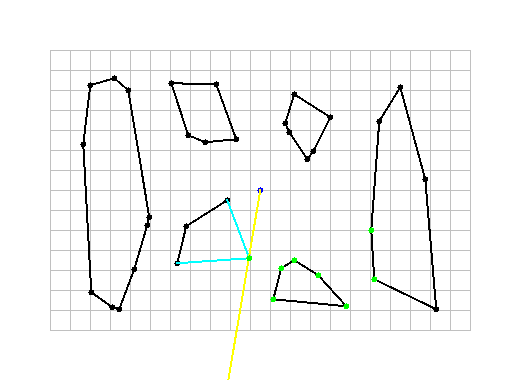
\includegraphics[width=7cm]{capture1}
}
\subfigure{
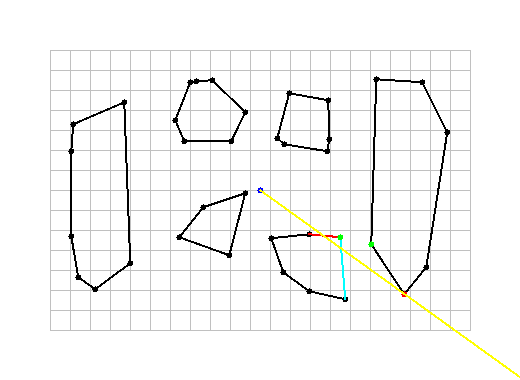
\includegraphics[width=7cm]{capture2}
}
\end{center}
\caption{Rotational Sweep}
\label{fig:12.2.a.1}
\end{figure}

\subtask{b}
Der Rest ist leicht: Der Sichtbarkeitsgraph entsteht aus der Anwendung des Sweep für jede Ecke aller Polygone. Bei insgesamt $n$ Ecken benötigt das folglich $O(n^2\cdot\log n)$ Zeit und $O(n^2)$ Platz für das Speichern des Graphen.

Interessant ist hier lediglich, welcher Punkt als Ausgangspunkt für den Strahl gewählt wird - der Sweep funktioniert in unserer Implementierung nicht für Punkte innerhalb eines Polygons (auch nicht auf dem Rand!). Gerade unter Berücksichtigung von Rundungsfehlern wären hier einige Spezialfälle zu behandeln wann inzidente Kanten die Sicht blockieren oder eben nicht.

Wir haben es uns hier ein wenig leicht gemacht: da wir ohnehin nur eine gewisse Präzison gewährleisten können (aufgrund der oben erwähnten Probleme mit Ungenauigkeiten bei der Sortierung des Baums) können wir auch hier eine kleine Ungenauigkeit erlauben und $p_l$ einfach ein kleines Stück von seinem Polygon ''wegschieben''. Hiermit sind - bei sehr kleinem Aufwand - alle Rundungs- und sonstigen Ungenauigkeiten erledigt und die möglichen Abweichungen in der Ergebnismenge fallen ohnehin in einen Bereich der schon aufgrund der Ungenauigkeit des Sweeps hingenommen werden muss.

Auf die (kürzesten) Wege hat diese Heuristik keine Auswirkung, da hierfür wieder die Original-Punkte (statt der verschobenen) genutzt werden.

Im Fall einer Ungenauigkeit kann ein Punkt der (annähernd) kollinear zu einer nicht inzidenten Kante ist als sichtbar erkannt werden, obwohl er es knapp nicht ist.

\lstinputlisting[language=Java, firstline=20, lastline=83]{../../AlGeo/src/geometry/algorithms/VisibilityGraph.java}

Abbildung \ref{fig:12.2.b.1} zeigt zwei aufeinanderfolgende Schritte im Algorithmus:
\begin{itemize}
\item Grün: Ergebnis des Sweeps für eine Ecke $v_i$
\item Rot: Ergebnisse der bisherigen Sweeps aller Ecken $v_1,...,v_{i-1}$
\end{itemize}

\begin{figure}[h!]
\begin{center}
\subfigure{
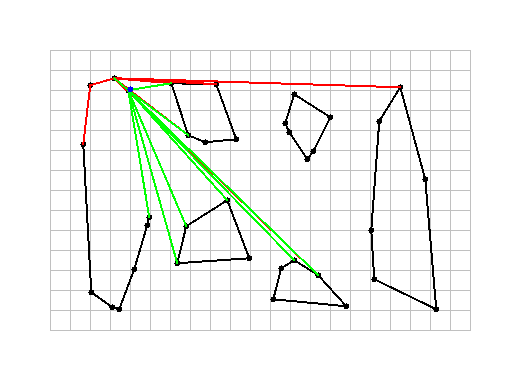
\includegraphics[width=7cm]{capture3}
}
\subfigure{
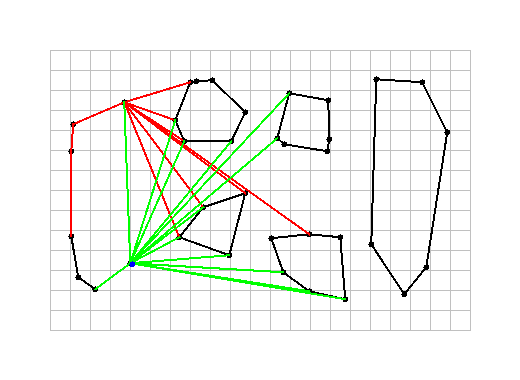
\includegraphics[width=7cm]{capture4}
}
\end{center}
\caption{Sichtbarkeitsgraph}
\label{fig:12.2.b.1}
\end{figure}

\subtask{c}
Warum einen berechnen, wenn man alle berechnen kann? Da der Anwendungsfall nicht näher spezifiziert ist (und ich sowieso noch eine alte Implementierung griffbereit habe ;) ) machen wir keinen Dijkstra (wie ggf. vom Autor der Aufgabe angedacht) sondern einen Floyd-Warshall um \emph{all-pairs-shortest-paths} zu berechnen. Im schlimmsten Fall (der Sichtbarkeitsgraph ist vollständig) benötigt man hierfür $O(n^3)$ Zeit und erneut $O(n^2)$ Platz. Abbildung \ref{fig:12.2.c.1} zeigt exemplarisch zwei dieser Wege.

\lstinputlisting[language=Java, firstline=15, lastline=18]{../../AlGeo/src/geometry/algorithms/VisibilityGraph.java}
\lstinputlisting[language=Java, firstline=85, lastline=156]{../../AlGeo/src/geometry/algorithms/VisibilityGraph.java}
\begin{figure}[h!]
\begin{center}
\subfigure{
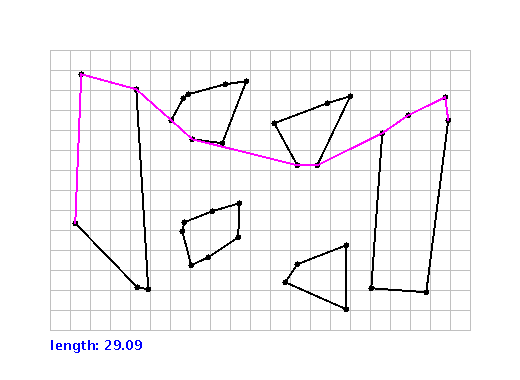
\includegraphics[width=7cm]{capture5}
}
\subfigure{
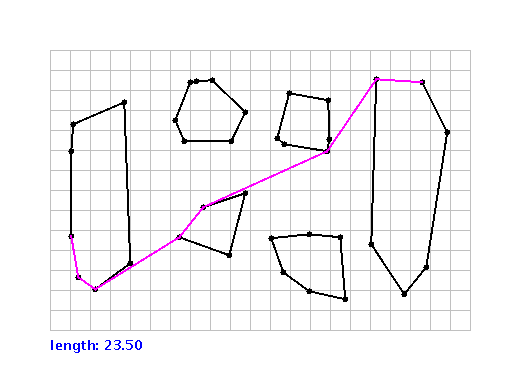
\includegraphics[width=7cm]{capture6}
}
\end{center}
\caption{Kürzester Weg}
\label{fig:12.2.c.1}
\end{figure}
\end{task}
\end{document}